\documentclass{article}

\usepackage[english]{babel}
\usepackage{blindtext}
\usepackage{microtype}
\usepackage{graphicx}
\usepackage{wrapfig}
\usepackage{enumitem}
\usepackage{fancyhdr}
\usepackage{amsmath}
\usepackage{chemformula}
\usepackage{index}
\usepackage{hyperref}
\usepackage[margin=1.0in]{geometry}
\usepackage{qtree}
\usepackage{tikz-qtree}
\usepackage{float}

\begin{document}
\title{Summary: Control of Body Temperature and Water Balance}
\author{Dowland Aiello}
\date{April 1, 2020}

\maketitle
\tableofcontents
\fancyhf{}

\newpage

\section{Mechanisms for maintaining homeostasis in climatically volatile conditions}

There exist various permutations, or implementations, if you will, of the
general principle of \emph{thermoregulation}---the mechanism through which an
internal temperature can be restricted to an acceptable range conducive to the
survival of a host. Two of these ``implementations'' may be described as
such\footnote{It is not uncommon for an animal to utilize both endothermic and
ectothermic heat regulation mechanisms. Take, for example, the
\href{https://en.wikipedia.org/wiki/Gentoo_penguin}{Pygoscelis papua}---a
member of the Penguin family---. While these birds do regulate body temperature
in a largely endothermic manner, they do warm themselves in the sun. This is an
example of both endothermic and ectothermic behavior. The same is true for the
ectothermic lizard.}:

\begin{itemize}
	\item \textbf{Endothermic heat regulation}: body heat is derived from the metabolic systems already posessed by a host.
	\item \textbf{Ectothermic heat regulation}: body heat is derived from an external source.
\end{itemize}

\subsection{Methods of heat exchange}

As does thermoregulation, the act of \emph{heat exchange} can occur in one of
several ways:

\begin{itemize}
	\item \textbf{Conduction}: the transfer of heat between objects that are in
		direct contact with each other.
	\item \textbf{Radiation}: the emission of electromagnetic waves, which can
		transfer heat between objects that are not in direct contact.
	\item \textbf{Convection}: the trnasfer of heat by the movement of air or
		liquid over a surface.
	\item \textbf{Evaporation}: the vaporization of molecules from the surface of a liquid.
\end{itemize}

\subsection{A demonstration of heat exchange}

Each of these disambiguations rely on the principle that heat flows from
an object of higher temperature to one of lower temperature. Yet, they
each serve unique purposes. For example, suppose an ecothermic lizard houses
itself atop a warm rock. The aforementioned modes of heat exchange operate on
the body temperature of the lizard in four ways:

\begin{enumerate}
	\item \emph{Conductively} --- Heat is transfered between the surface of the
		rock and the scales of the lizard through the immediate contact
		established between the rock and the lizard.
	\item \emph{Radiatively} --- Energy from the sun warms the
		lizard's back. Furthermore, heat is released from the lizard itself,
		in much the same manner, into the environment.
	\item \emph{Convectionally} --- A breeze lifts heat from the
		lizard's tail.
	\item \emph{Evaporatively} --- Moisture evaporates from the
		nostrils of the lizard.
\end{enumerate}

\begin{figure}[ht]
	\centering
	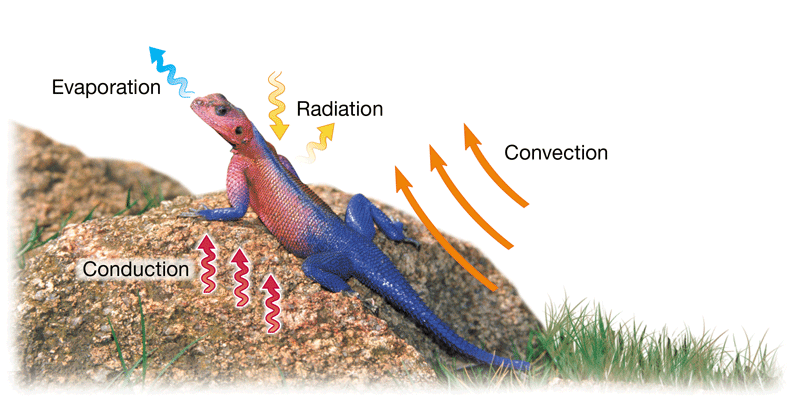
\includegraphics[width=6cm]{lizard_example.png}
	\caption{The lizard from our example}
\end{figure}

\pagebreak

\section{Notable thermoregulation adaptations}

\subsection{Classifications of thermoregulation adaptations}

While the aformentioned principle of temperature regulation, or
\emph{thermoregulation} can be grouped into two disambiguations: endothermism
and ectothermism, five common implementations of thermoregulation can be
derived from these larger categorizations. More specifically, the 
aforementioned five distinct categorizations are described as such:

\begin{enumerate}
	\item \textbf{Metabolic heat production}: energy is release as heat---a
		byproduct of ATP synthesis processes. In humans, this results in a warm
		feeling while exercising. In hibernating mammals, on the other hand,
		ATP synthesis and warming processes are decoupled (e.g., hibernating
		bears).
	\item \textbf{Insulation}: hair/fur, feathers, and fat reduce the
		radiation of heat from an animal to its environment.
	\item \textbf{Circulatory adaptations}: when surface blood vesssels are
		constricted, the rate of heat loss through radiation is reduced as a
		result of a lowered volume of blood flowing to the cold surface.
		\emph{Countercurrent heat exchange} is an example of a circulatory
		adaptation found in the limbs of many birds and mammals.\footnote{This
		technique describes the tendency for warm and cold blood to flow in
		opposite directions in adjacent vessels, and should not be confused with
		\emph{concurrent} exchange. One should recall: countercurrent exchange
		provides utility to an organism by conductively exchanging heat between
		warm blood moving towards the outer regions of the corpus and cold blood
		moving back to the warm core of the organism in question.}

	\item \textbf{Evaporative cooling}: water absorbs heat from the surface of
		the body (e.g., as sweat evaporates, heat is lost).
	\item \textbf{Behavioral responses}: an animal's internal temperature is
		controlled through an adjustment to the animal's behavior. For example,
		humans dress more heavily in colder environments.
\end{enumerate}

\begin{figure}[h]
	\centering
	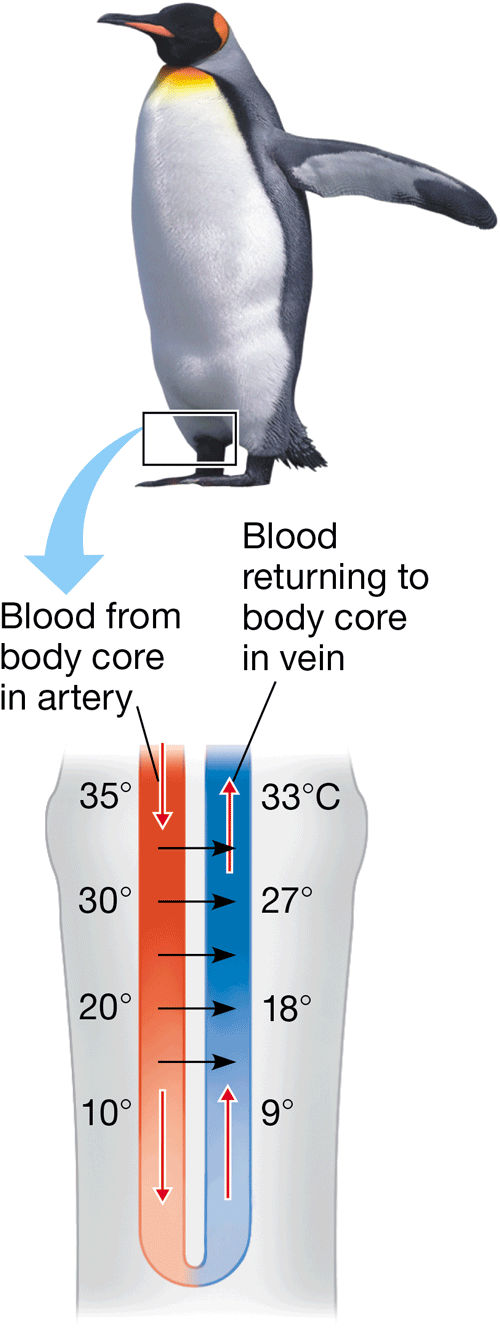
\includegraphics[width=2cm]{penguin_example_ccexchange.png}
	\caption{A penguin, countercurrently exchanging heat}
\end{figure}

\subsection{Application of thermoregulation in huddles of penguins}

Through a behaivoral response-mediated thermoregulation adaptation, huddles of
penguins are able to converse energy otherwise lost through radiation and
convection. As is the case in a single penguin, in a huddle of penguins, the
largest concentration of heat is present in the core of the complex, while the
least amount of heat is present in the edges of the huddle. In order to
maximize the effectivity of this strategy and minimize losses to the poorly-
insulated periphery, all members of the ``huddle'' will eventually serve as the
huddle's ``core.'' This theory was demonstrated in \href{https://www.wired.com/2011/06/penguins-shuffle-warm/}{a 2011 German study}
conducted on a huddle of emperor penguins.

\section{Osmoregulation and excretion}

\subsection{Why osmoregulation and excretion mechanisms are necessary}

As is the case with internal temperatures, in order to maintain homeostatis,
organisms must maintain a healthy balance of water and solutes. In the case of
an \emph{osmoconformer}, this is a rather straightforward task. An osmoconformer
is, by specification, of an isotonic solute concentration\footnote{Common
examples of osmoconformers are: jellies, molluscs, squids, and sea stars.}.
\emph{Osmoregulators}, on the other hand, maintain homeostatis not by
construction, but by correction: through \textbf{osmoregulation}, an
osmoregulator is able to prevent the loss of water or of a certain solute.

\begin{figure}[h]
	\centering
	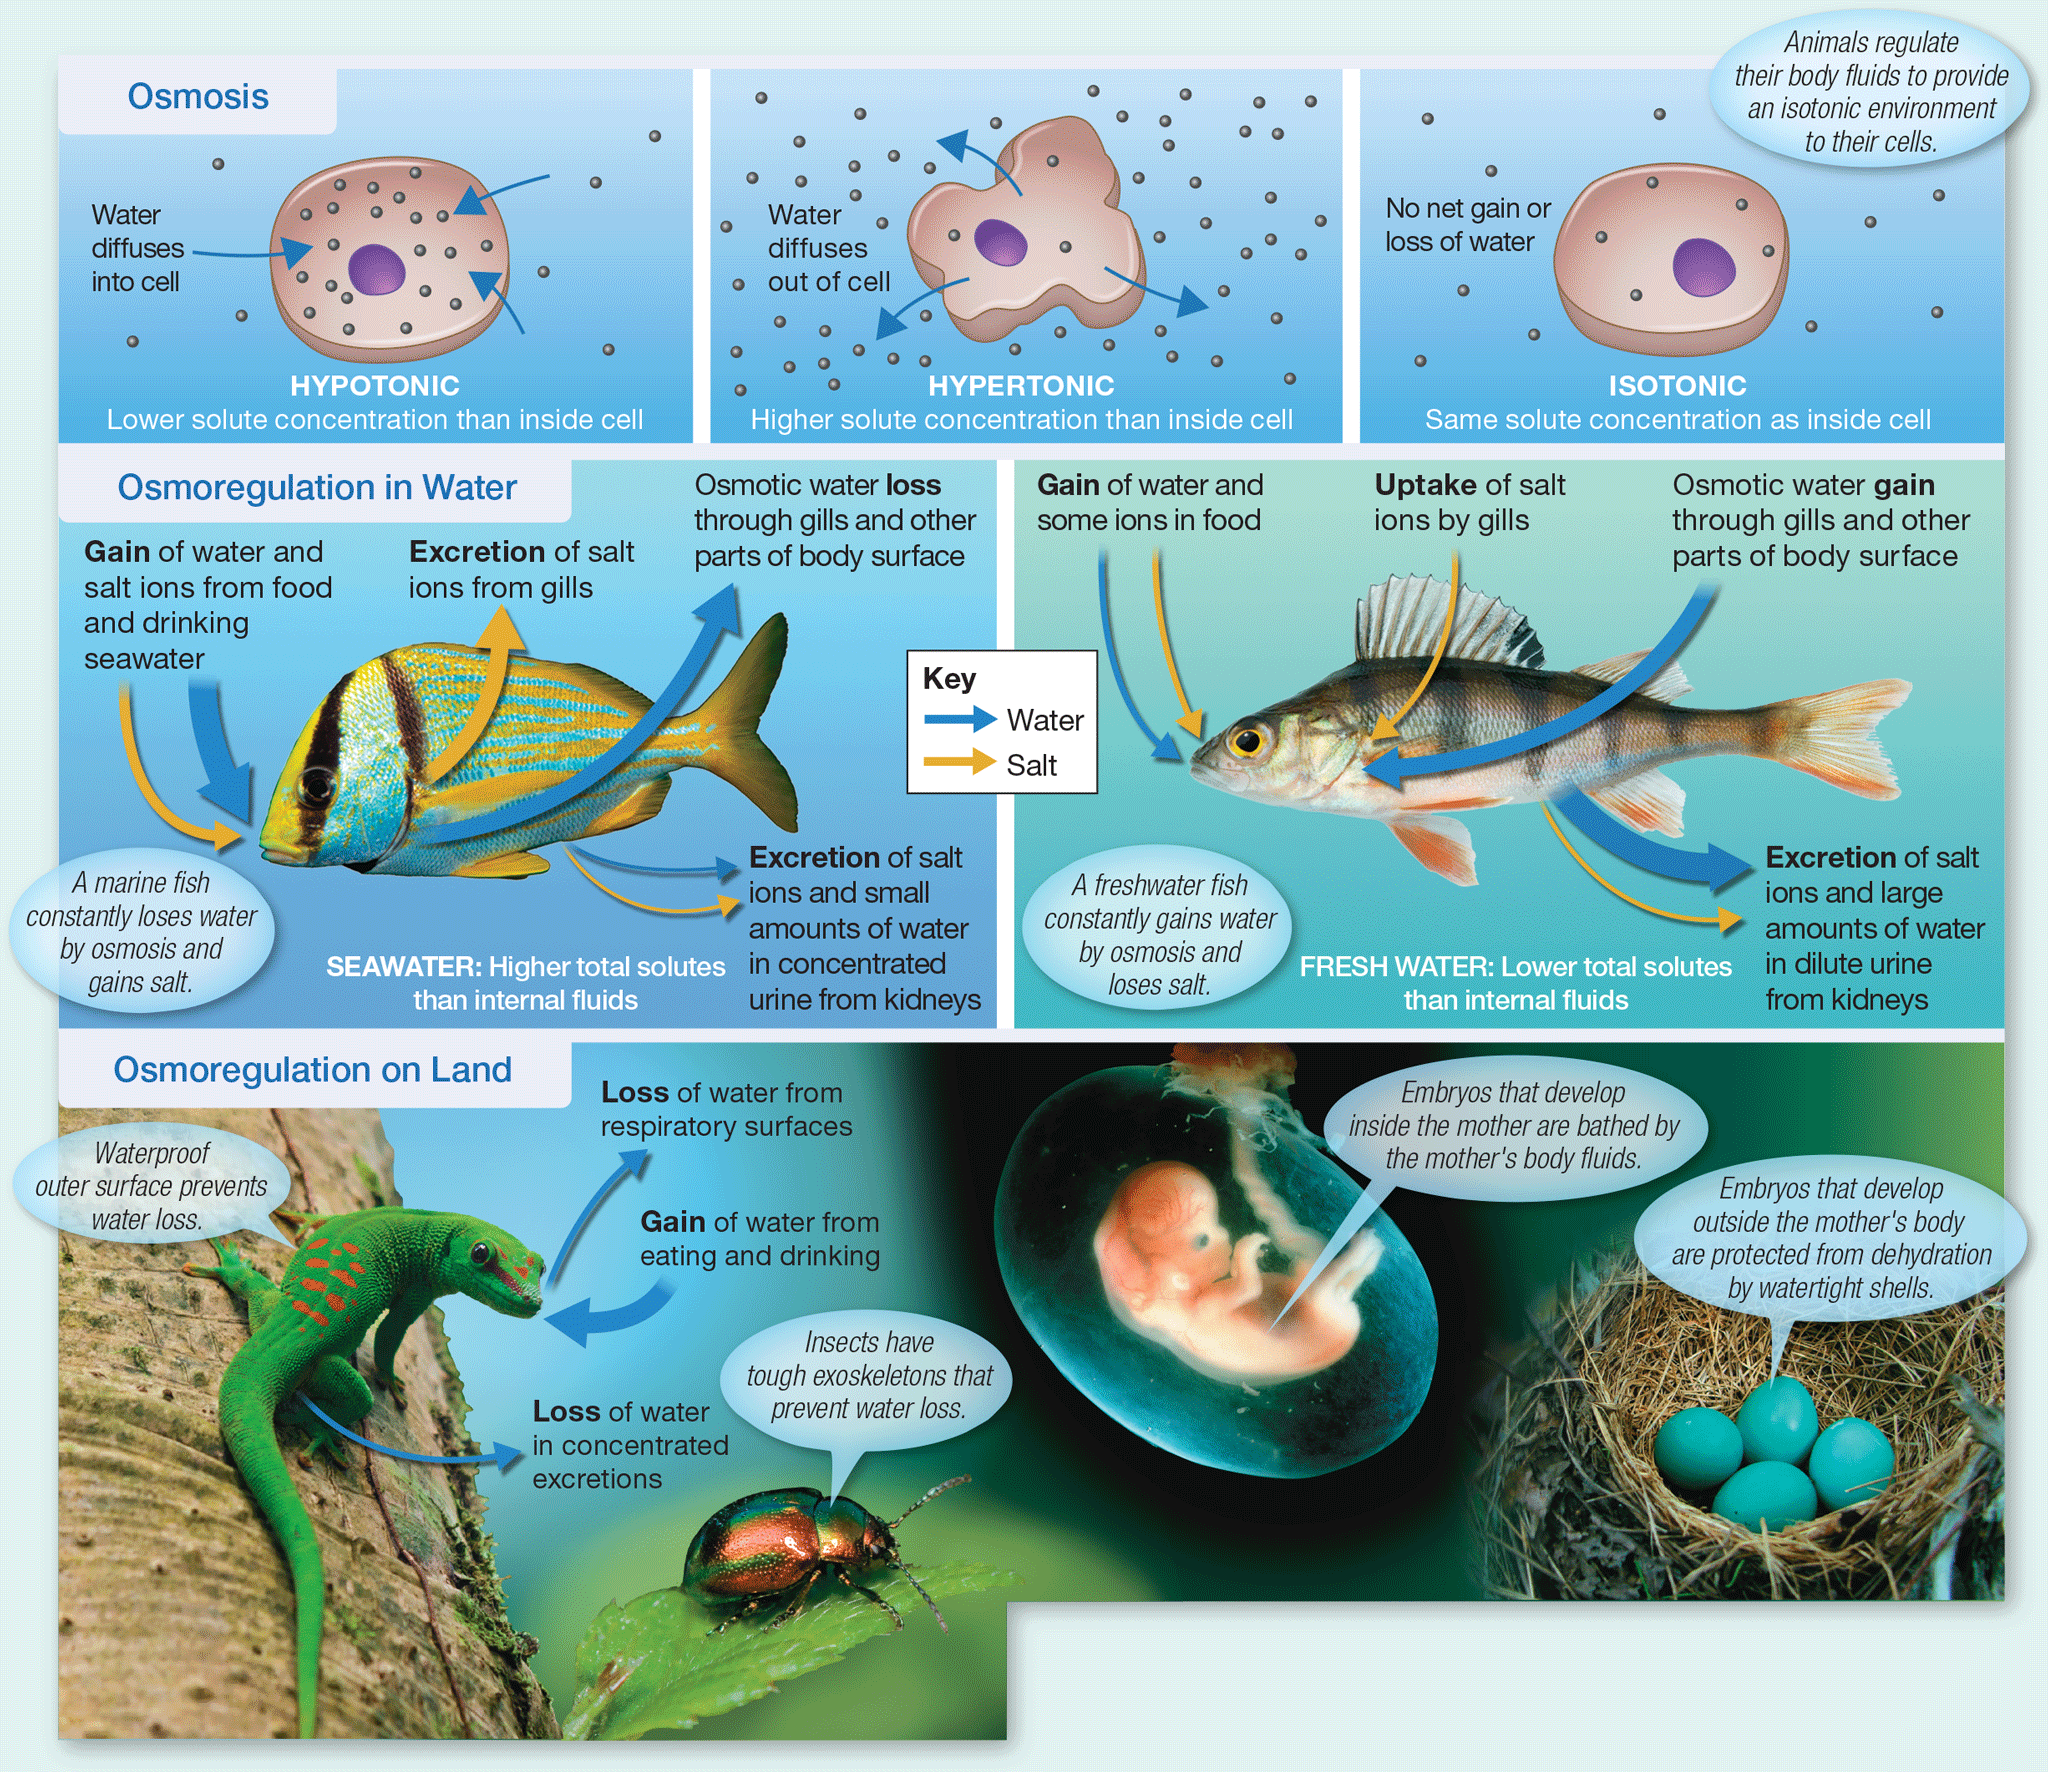
\includegraphics[width=15cm]{types_of_osmo.png}
	\caption{The various types of osmoregulating organisms, and the mechanisms
	on which they depend.}
\end{figure}

\subsection{Excretion deals with waste disposal}

Though it is objectively differentiated from the aforementioned principle of
osmoregulation, excretion is tightly coupled in its implementation of waste
disposal: in order to purge the body of some particular waste, such waste must
be expelled to a body of water. But, more generally, \textbf{excretion} can
simply be defined as the disposal of metabolic waste. Of course, the material
being expelled, and how such material is expelled is a matter of developmental
preference. Common metabolic wastes of animals can be defined as such:

\begin{itemize}
	\item \textbf{Ammonia} (\ch{NH3}): highly soluble and diffuses rapidly. In
		acquatic animals, this property is rather appealing, as it allows for
		the passive disposal of this toxic chemical into the surrounding
		environment. In order to be transported actively, Ammonia must be
		heavily diluted, due to its toxic nature. This amount of unused water
		is often unattainable in terrestrial animals. As such, Ammonia is often
		converted, rather than transported in terrestrial animals.
	\item \textbf{Urea} (\ch{CH4N2O}): a major waste product excreted by mammals,
		adult amphibians, sharks, and bony fishes. Urea is produced in the liver
		through the combination of \ch{NH3} with \ch{CO2}, and can be
		substituted for Ammonia in excretion.
	\item \textbf{Uric Acid} (\ch{C5H4N4O3}): a target for Ammonia conversion
		in various repitles, birds and insects. The conversion of Ammonia to
		uric acid is often appealing, as it can offset water loss almost
		completely, and is relatively nontoxic. However, the excretion of this
		waste in its ``semisolid paste'' form consumes a fair amount of energy,
		but is still appealing considering the water savings with respect to
		the alternative: urea.
\end{itemize}

\subsection{Excretion, filtration, and osmoregulation in humans}

\subsubsection{The role of the kidneys in homeostasis}

In order to preserve the greatest amount of both water and nutrients possible,
humans refrain from excreting all of the \textbf{filtrates}---a combination of
water, nutrient solutes and urea---present in our blood\footnote{About 180 L of
filtrate is collected by the kidneys each day.}. Instead of simply purging the
body of all filtrates, filtrates are first collected by the kidneys, which
return water and nutrients back to the blood. About 1.5 L of \textbf{urine},
a refined, more heavily concentrated form of urea, is produced by the kidneys
each day.

\subsubsection{The pathway of filtrate and urine}

In order for urine to be filtered by the kidneys, blood must first enter the
kidney through the \textbf{renal artery}. As is implied by its name, blood will
eventually exit the kidney through the \textbf{renal vein}. Generally, the
pathway taken by blood from the bloodstream, into the kidney, and back is as
follows:

\begin{enumerate}
	\item Blood enters the kidney via the renal artery.
	\item Filtrate is forced into a capillary wall, and into a kidney tube by
		the pressure of moving blood.
	\item Urine leaves the kidney through the \textbf{ureter}.
	\item Blood leaves the kidney through the renal vein.
	\item Urine is drained from the ureter into the \textbf{urinary bladder}
	\item Urine is expelled from the bladder through the \textbf{urethra},
		where the \textbf{sphincter} controls the flow of urine.
\end{enumerate}

\begin{figure}[h]
	\centering
	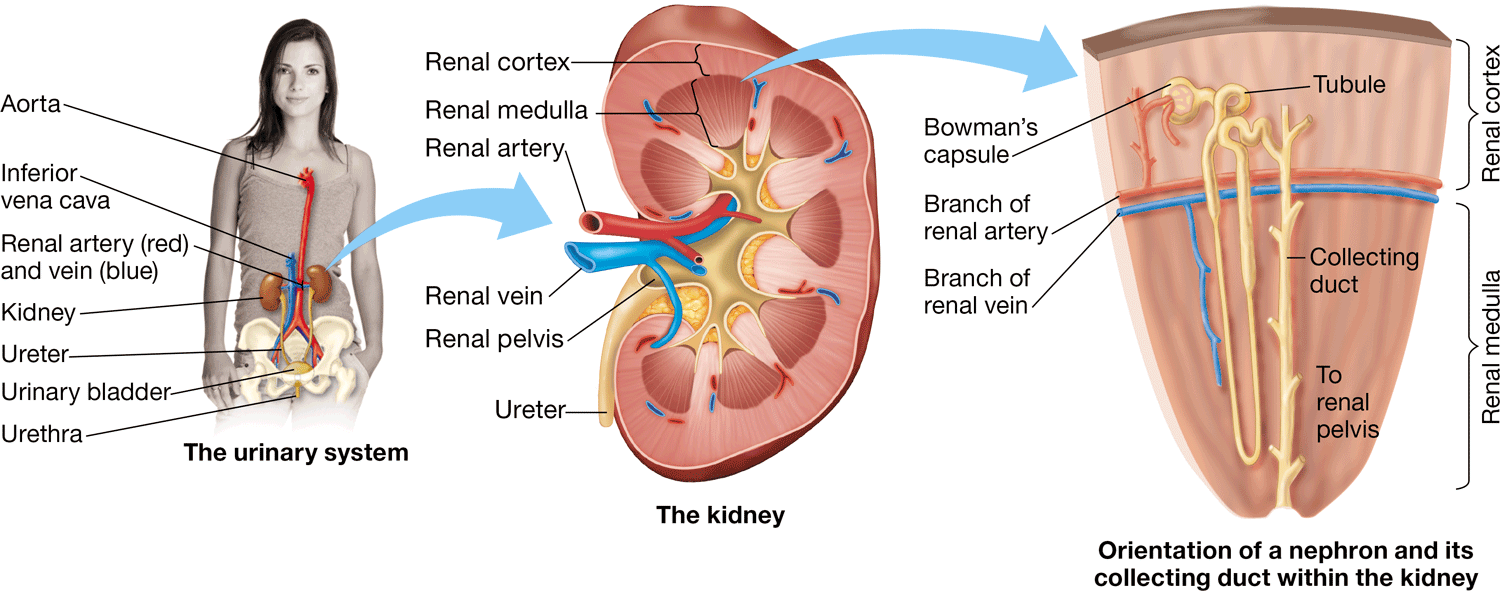
\includegraphics[width=8.5cm]{urinary_system.png}
	\caption{The human urinary system}
\end{figure}

\subsection{The structure of the kidney}

The highest level components of the kidney lie in the organ's division into two
main compartments: the \textbf{renal cortex} and the inner \textbf{renal
medula}. Inside the renal medula, millions of \textbf{nephrons} process
filtrate in parallel. A nephron consists of:

\begin{itemize}
	\item A single folded tubule
	\item Associated blood vessels
\end{itemize}

These two components of the nephron can be further described in terms of their
position with respect to the kidney and their function. For example, the
\textbf{bowman's capsule} is a term used to refer to the cup-shaped
blood-filtering end of the nephron. The function of a nephron has been carried
out once it disposes of its refined filtrate into the \textbf{collecting duct}
of the cortex, which carries urine to the renal pelvis. 

Before one analyzes the flow of blood and filtrates in the nephron, one must
first recognize the three sections of the nephron in which filtrate processing
occurs:

\begin{enumerate}
	\item The \textbf{promixal tubule}: conveys and helps refine filtrate.
	\item The \textbf{Loop of Henle}: helps concentrate the filtrate conveying
		it between a proximal tubule and a distal tubule
	\item The \textbf{Distal tubule}: helps refine filtrate and empties it into a
		collecting duct
\end{enumerate}

Inside of the nephron, blood and filtrate will take the following path:

\begin{center}
	\Tree[.{Both enter renal artery} [.{Both enter glomerulus} [.{Blood remains in capillaries} [.{Blood exits Bowman's capsule via arteriole} [.{Various capillaries} [.{Renal vein} ] ] ] ] 
															   [.{Filtrate enters nephron tube} [.{Proximal tubule} [.{Loop of Henle} [.{Distal tubule} [.{Collecting duct} ] ] ] ] ]]]
\end{center}

Even after filtrates are processed in the nephrons, the process of
\textbf{reabsorption} serves to further process the products of the
aforementioned process by returning nutrients to the blood through capillary
walls. \textbf{Secretion}, on the other hand, can be used to remove unwanted
minerals from the bloodstream via the filtrate products of the nephron
processes.

\begin{figure}[H]
	\centering
	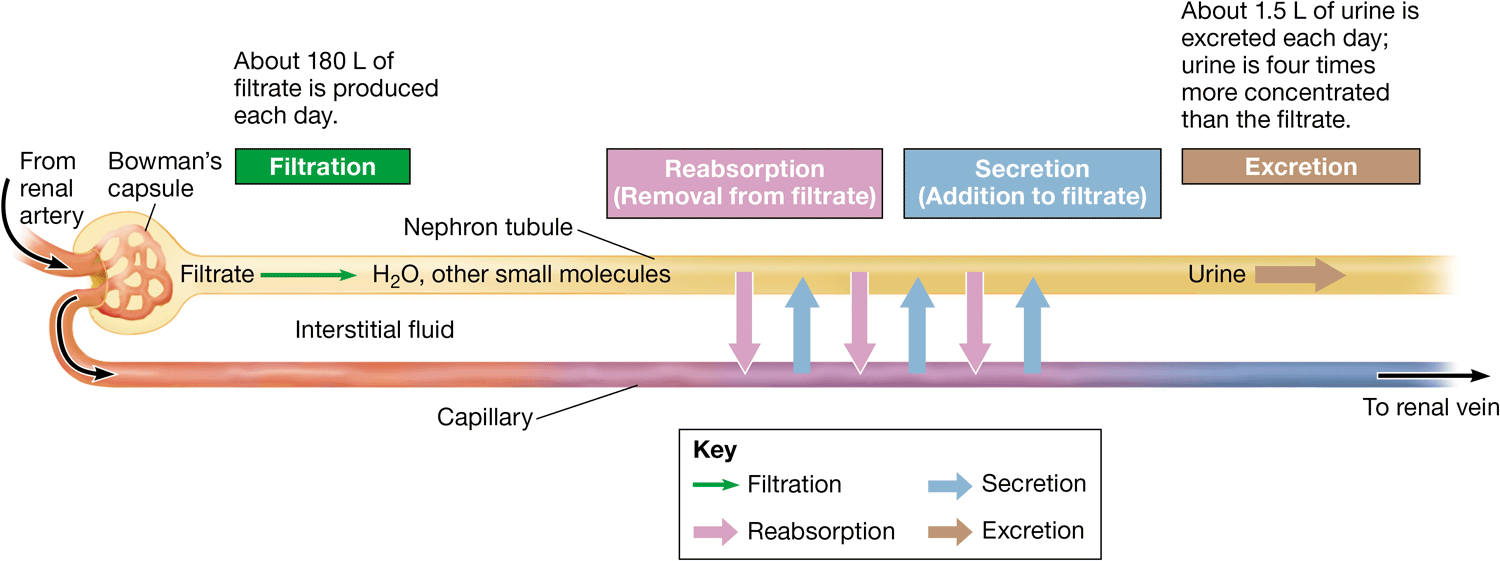
\includegraphics[width=8cm]{secondary_processes.png}
	\caption{The relationship between the nephron and secretion/reabsorption}
\end{figure}


Once initial processing and secretion/reabsorption have completed, urine is
excreted from the body via the ureters, urinary bladder, and urethra.

\begin{figure}
	\centering
	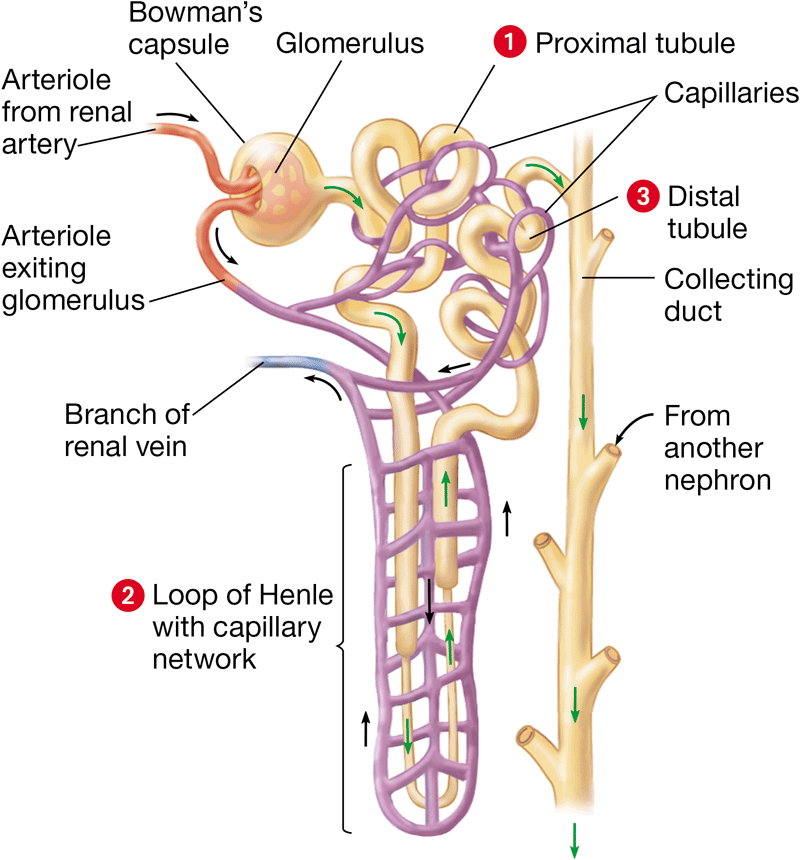
\includegraphics[width=8cm]{nephron_structure.png}
	\caption{The pathway of blood and filtrates through the nephron}
\end{figure}

\end{document}
